\documentclass[journal]{IEEEtran}

\usepackage{cite}
\usepackage{amsmath,amssymb}
\usepackage{graphicx}
\usepackage{booktabs}
\usepackage{xurl}
\usepackage[hidelinks]{hyperref}
\emergencystretch=2em
\renewcommand{\topfraction}{0.9}
\renewcommand{\bottomfraction}{0.8}
\renewcommand{\textfraction}{0.07}
\renewcommand{\floatpagefraction}{0.85}
\renewcommand{\dbltopfraction}{0.9}
\renewcommand{\dblfloatpagefraction}{0.85}
\setcounter{topnumber}{3}
\setcounter{dbltopnumber}{2}
\setcounter{totalnumber}{4}

\newcommand{\R}{\mathbb{R}}
\newcommand{\Lbase}{\mathcal{L}_{\mathrm{base}}}
\newcommand{\Lglobal}{\mathcal{L}_{\mathrm{gSC}}}
\newcommand{\Lpart}{\mathcal{L}_{\mathrm{pSC}}}
\newcommand{\Lptrip}{\mathcal{L}_{\mathrm{pTri}}}
\newcommand{\tablesetup}{\footnotesize\setlength{\tabcolsep}{4pt}}

\begin{document}

\title{Part Supervision Versus Part Matching for Pose-Based Gait Recognition Under Missing Joints}

\author{Minas~Aslanyan and Levon~Aslanyan%
\thanks{M. Aslanyan and L. Aslanyan are with the Institute for Informatics and
Automation Problems, National Academy of Sciences of the Republic of Armenia,
Yerevan, Armenia (e-mail: minas.aslanyan@iiap.sci.am; lasl@sci.am).
Corresponding author: Minas Aslanyan.}%
\thanks{This research did not receive any specific grant from funding agencies
in the public, commercial, or not-for-profit sectors.}}

\markboth{IEEE Transactions on Biometrics, Behavior, and Identity Science}%
{Aslanyan and Aslanyan: Part Supervision Versus Part Matching for Pose-Based Gait Recognition}

\maketitle

\begin{abstract}
Part-aware pose-based gait recognizers usually combine two interventions:
identity objectives on body regions during training and fusion of regional
similarities during retrieval. We separate them on one fixed multistream graph
encoder for two-dimensional poses and then test the result on GPGait. On
CASIA-B development identities, seven training objectives, including global
and part supervised contrastive (SupCon) terms and cross-entropy controls, were
each trained with five seeds and evaluated under synthetic missing joints. No
auxiliary contrastive objective differed reliably from a metric-learning
baseline; an initial three-seed part-SupCon penalty ($-6.12$ Rank-1 points,
95\% interval $[-10.29,-2.00]$) shrank to $-1.27$ $[-5.24,2.74]$. Fusing
normalized raw part pools from frozen checkpoints instead improved
corrupted-probe Rank-1 under every objective ($+2.32$ to $+4.28$ points), and
controls located the gain in score fusion rather than in learned heads or
confidence weighting. On Gait3D test identities, evaluated once with a frozen
recipe, the matcher raised Rank-1 from 21.88\% to 23.86\% ($+1.99$
$[0.61,3.38]$), level with GPGait reproduced on identical data (23.13\%). The
gain did not transfer to GPGait itself: its trained part branches added 9.08
points on CASIA-B and 5.17 on Gait3D, whereas adding raw parts lowered accuracy
by 2.40 and 3.17 points. Our encoder also remains far below GPGait on CASIA-B
(54.04\% versus 80.91\%). Whether local supervision or local matching carries a
part-aware gain therefore depends on the encoder, and both should be measured
on the same frozen checkpoints.
\end{abstract}

\begin{IEEEkeywords}
Biometrics, gait recognition, occlusion robustness, part-based matching, pose estimation, supervised contrastive learning.
\end{IEEEkeywords}

\section{Introduction}
\label{sec:introduction}

Pose-based gait recognition retrieves identities from joint trajectories. The
representation is compact and depends less on clothing, background and
illumination than silhouettes do \cite{liao2020posegait}, and graph encoders
such as ST-GCN, GaitGraph and GaitGraph2 make its spatial and temporal
structure explicit \cite{yan2018stgcn,teepe2021gaitgraph,teepe2022gaitgraph2}.
Recognition is nevertheless limited by what the pose estimator recovers.
Occlusion and detector failures remove joints or produce wrong tracks, so
partial body evidence is a central difficulty \cite{li2024survey,huang2024occluded}.

Body regions offer two distinct interventions. During training, a local
identity objective can push each region to discriminate individuals. During
retrieval, regional similarities can supplement a global sequence score.
Part-aware systems usually adopt both at once, yet a region can contribute
useful complementary matching evidence without being independently
discriminative under a local loss. Supervised contrastive (SupCon) learning
\cite{khosla2020supervised} offers a natural local objective, but whether it
helps gait parts is an empirical question. Attributing an improvement to the
intended mechanism requires separating the two interventions.

We perform that separation on one fixed multistream graph encoder whose input
representation, augmentation, batches, base losses, checkpoint selection and
evaluation masks are shared; only the auxiliary objective or the retrieval
descriptor changes. No auxiliary global or part SupCon term reliably improves
a metric-learning baseline, and a part-SupCon penalty seen in an initial
three-seed factorial is much smaller with five seeds. Matching normalized raw
part pools from the same frozen checkpoints improves corrupted-probe accuracy
under every objective and on both CASIA-B and Gait3D, including Gait3D test
identities evaluated once with a recipe frozen beforehand. Weighting parts by
detector confidence adds nothing over uniform averaging. The result does not
transfer to GPGait \cite{fu2023gpgait}, whose part-specific branches are trained
with their own losses: there the trained parts add 5 to 9 points and raw part
matching lowers accuracy (Fig.~\ref{fig:summary}). The contributions are:
\begin{enumerate}
    \item A controlled comparison of global and part SupCon, cross-entropy
    controls and a metric-learning baseline on one pose-gait encoder, with a
    five-seed replication that revises a three-seed finding.
    \item Checkpoint-only controls (raw pools, uniform weights, ten random heads,
    five fusion weights) and raw matching for every trained objective, which
    locate the retrieval gain in regional score fusion.
    \item An external Gait3D evaluation with a recipe frozen before test access,
    a detector-confidence stratification, and GPGait and GaitGraph2 reproduced on
    identical data.
    \item A transfer test on GPGait showing that its trained part branches, not
    training-free regional matching, carry its part-aware gain.
\end{enumerate}
Which part intervention helps therefore depends on the encoder, and the design
check we recommend is to compare global, raw regional and trained regional
matching on the same frozen checkpoints before crediting either one.

\begin{figure}[!t]
\centering
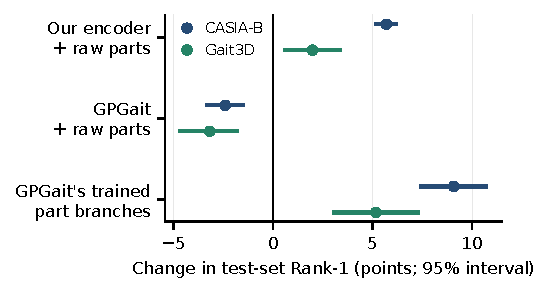
\includegraphics[width=\columnwidth]{fig1.pdf}
\caption{Test-set Rank-1 change from regional evidence. Training-free raw part
matching helps our encoder on CASIA-B (standard protocol, five seeds, paired $t$
interval) and Gait3D (five seeds, crossed bootstrap) but lowers the accuracy of
GPGait, whose trained part branches carry a large gain instead (one model per
dataset; intervals resample test identities).}
\label{fig:summary}
\end{figure}

\section{Related work}
\label{sec:related}

\paragraph{Contrastive and metric objectives}
Contrastive objectives depend on positive-pair construction and projection
geometry \cite{chen2020simclr,he2020moco,khosla2020supervised}, which can be
described by alignment and uniformity \cite{wang2020alignment}; other
self-supervised objectives avoid negatives or regularize variance and
redundancy \cite{grill2020byol,chen2021simsiam,zbontar2021barlow,bardes2022vicreg}.
Skeleton-specific contrastive learning serves action recognition and
re-identification \cite{thoker2021skeleton,rao2024skeleton,lin2023actclr} and
large-scale gait pretraining \cite{cosma2026gaitpt}. Sampling and pair weighting
shape metric objectives \cite{wu2017sampling,wang2019multisimilarity}, loss
comparisons require matched training and evaluation \cite{musgrave2020reality},
and interactions between losses can be inspected through their gradients
\cite{sener2018multiobjective,yu2020gradient}. None of these results determines
whether an independent identity objective helps each anatomical gait region.

\paragraph{Pose-gait encoders and missing evidence}
PoseGait uses body pose and human priors \cite{liao2020posegait}, GaitGraph
and GaitGraph2 learn graph features \cite{teepe2021gaitgraph,teepe2022gaitgraph2},
GPGait adds part-aware local--global graph extraction \cite{fu2023gpgait}, and
SkeletonGait renders skeleton maps \cite{fan2024skeletongait}; OpenGait and
FastPoseGait standardize implementations \cite{fan2022opengait,meng2023fastposegait},
and skeleton action encoders offer further graph and heatmap designs
\cite{shi2019adaptive,li2019actional,liu2020msg3d,cheng2020shift,duan2022posec3d}.
Real occlusion combines missing joints with mislocalization
\cite{li2024survey,huang2024occluded,chen2023iopstl}, and GREW, Gait3D and
SUSTech1K supply unconstrained or occluded conditions
\cite{zhu2021grew,zheng2022gait3d,shen2023lidargait}.

\paragraph{Part-aware representations}
GaitSet pools silhouette sets, and disentangling methods separate identity from
appearance or covariates
\cite{chao2019gaitset,zhang2019disentangled,li2020disentangled}. GaitPart,
GaitGL and 3D local CNNs extract complementary local and global features
\cite{fan2020gaitpart,lin2021gaitgl,huang2021local}; strip-based,
context-sensitive temporal, dynamic-region and template representations
extend the aggregation choices
\cite{wang2022gaitstrip,huang2021cstl,wang2023dygait,huang2025template}.
These systems train and match local features together. We claim no novelty
for anatomical pooling or global--local fusion; we ask which of the two carries
the gain, first with our encoder held fixed and then on GPGait.

\section{Study design}
\label{sec:design}

Figure~\ref{fig:framework} summarizes the design.

\begin{figure*}[!t]
\centering
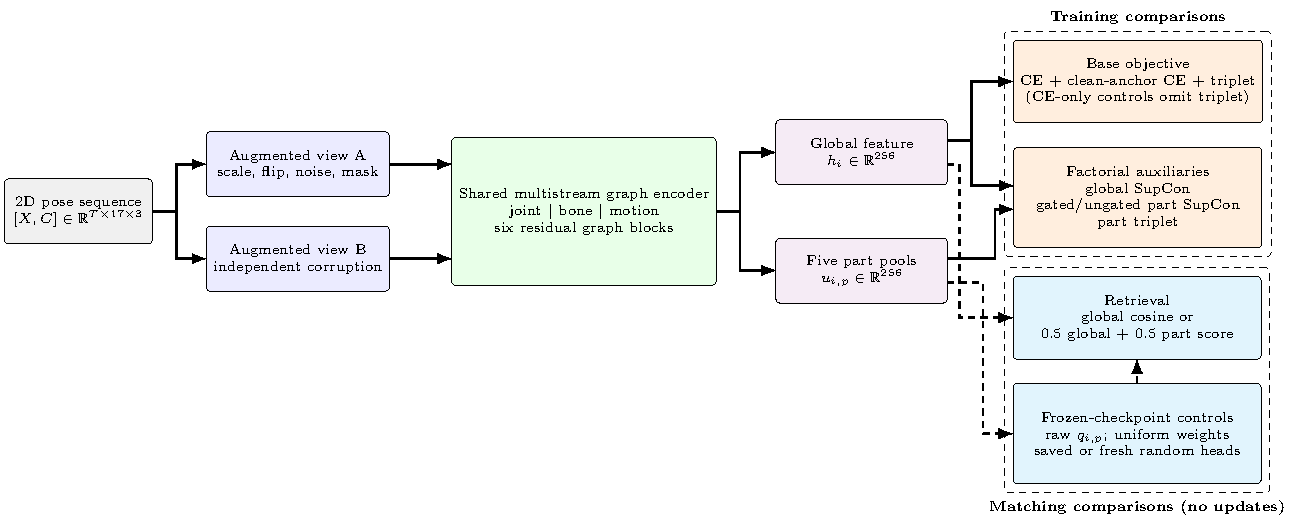
\includegraphics[width=\textwidth]{fig2.pdf}
\caption{Separation of part-aware training from part-aware matching. Solid
arrows denote the shared forward path. The upper branch contains the training
objectives; the lower branch contains frozen-checkpoint descriptor controls
and performs no parameter updates.}
\label{fig:framework}
\end{figure*}

\subsection{Encoder and regional descriptors}

Let $X\in\R^{T\times17\times2}$ be a normalized pose and $C\in[0,1]^{T\times17}$
its confidence. The encoder builds three input streams: joints $[X,C]$; bones
relative to a rooted parent, observed only when both endpoints are present; and
motion at lags one and two, observed only when both temporal endpoints are
present. Stream-specific stems feed six residual graph blocks that use learned
perturbations of the physical adjacency and temporal convolutions with
dilations 1, 2 and 4. The width grows from 64 to 256, and confidence-weighted
global pooling gives a normalized 256-dimensional embedding $h_i$.

Five overlapping COCO regions define local pools: the torso (shoulders and
hips), two arms (shoulder, elbow, wrist) and two legs (hip, knee, ankle); face
joints are excluded. Confidence-weighted pooling within part $p$ gives
$u_{i,p}\in\R^{256}$. The deterministic raw descriptor is
$q_{i,p}=u_{i,p}/\lVert u_{i,p}\rVert_2$; the learned alternative passes
$u_{i,p}$ through a part-specific two-layer head and $\ell_2$ normalization to
give $z_{i,p}$. Part reliability is
\begin{equation}
 r_{i,p}=\frac{1}{T_i|p|}\sum_{t=1}^{T_i}\sum_{j\in p}C_{i,t,j},
 \label{eq:reliability}
\end{equation}
where $T_i$ counts real rather than padded frames.

\subsection{Training objectives}

Each batch samples 16 identities with four sequences each. For matched CE, the
metric baseline and every auxiliary variant, two views of each sequence receive
scale, flip and coordinate-noise augmentation; each view
independently stays geometrically complete with probability 0.3 and otherwise
receives random-joint, body-part or temporal masking, with the maximum
severity rising linearly from 0.05 to 0.5 over the first half of training.
Dynamic-joint corruption is reserved for evaluation. The metric baseline uses
\begin{equation}
 \Lbase = \mathcal{L}_{\mathrm{CE,aug}} + 0.5\,\mathcal{L}_{\mathrm{CE,clean}} + \mathcal{L}_{\mathrm{Tri}},
 \label{eq:base}
\end{equation}
where the first term classifies both augmented views, the clean anchor
classifies the unaugmented sequence, and $\mathcal{L}_{\mathrm{Tri}}$ is
batch-hard triplet loss \cite{hermans2017triplet} on $h_i$ with margin 0.2;
same-source views are excluded as triplet positives. Global SupCon $\Lglobal$
acts on a projection of $h_i$ with every same-identity view as positive. Part
SupCon $\Lpart$ applies the same construction to each $z_{i,p}$; in the gated
form a positive pair is weighted by $r_{i,p}r_{j,p}$ and the anchor by
$r_{i,p}$, and parts with reliability below 0.05 are excluded. The ungated form
gives every part above that threshold unit weight. Part triplet $\Lptrip$
applies batch-hard triplet loss to every present part. The full objective is
\begin{equation}
 \mathcal{L}=\Lbase+\gamma_g\Lglobal+\gamma_p\Lpart+\gamma_{pt}\Lptrip .
 \label{eq:objective}
\end{equation}
Table~\ref{tab:objectives} lists the configurations. Three CE controls bracket
the baseline: plain CE without masking, CE with random joint dropout, and
matched CE, which uses the baseline's partial views and clean anchor but no
triplet term.

\begin{table*}[!t]
\centering
\caption{Training objectives. All other settings are shared. ``Five'' and
``three'' mark the CASIA-B cohorts that contain each objective; Gait3D
development uses CE, matched CE, the metric baseline and global + part SupCon.}
\label{tab:objectives}
{\tablesetup
\begin{tabular}{@{}lcccccl@{}}
\toprule
Configuration & Triplet & $\gamma_g$ & $\gamma_p$ & $\gamma_{pt}$ & Part gate & CASIA-B seeds \\
\midrule
CE, no masking & -- & 0 & 0 & 0 & -- & five \\
Masked CE (joint dropout) & -- & 0 & 0 & 0 & -- & five \\
Matched CE & -- & 0 & 0 & 0 & -- & five \\
Metric baseline & \checkmark & 0 & 0 & 0 & -- & five, three \\
Global SupCon & \checkmark & 0.2 & 0 & 0 & -- & five, three \\
Part SupCon & \checkmark & 0 & 0.2 & 0 & reliability & five, three \\
Global + part SupCon & \checkmark & 0.2 & 0.2 & 0 & reliability & five, three \\
Global + part SupCon, ungated & \checkmark & 0.2 & 0.2 & 0 & presence & three \\
Part triplet & \checkmark & 0 & 0 & 0.2 & -- & three \\
\bottomrule
\end{tabular}}
\end{table*}


\subsection{Retrieval descriptors and checkpoint-only controls}

The global descriptor scores $s_g(i,j)=h_i^{\top}h_j$. A part descriptor keeps
this term and averages local cosine scores over jointly reliable parts. With
$v_{i,p}$ either the learned projection $z_{i,p}$ or the raw pool $q_{i,p}$,
\begin{align}
 s_p(i,j)&=\frac{\sum_p r_{i,p}r_{j,p}\,v_{i,p}^{\top}v_{j,p}}{\max\left(\sum_p r_{i,p}r_{j,p},10^{-8}\right)},\\
 s(i,j)&=(1-\lambda)\,s_g(i,j)+\lambda\, s_p(i,j),
 \label{eq:matching}
\end{align}
with $\lambda=0.5$ declared before any comparison. Uniform matching replaces
$r_{i,p}$ by the presence indicator $\mathbf{1}[r_{i,p}>0]$, and matching falls
back to $s_g$ when no part is jointly present. In the metric baseline and
global SupCon runs the part heads receive no loss, so their learned
projections stay at their seeded initialization while the backbone changes.
The checkpoint-only controls resolve this confound: each selected
metric-baseline checkpoint is frozen and evaluated with (i) raw pools and
reliability weights, (ii) raw pools and uniform weights, (iii) the saved
untrained heads and (iv) ten freshly initialized heads of the same
architecture, at $\lambda\in\{0,0.25,0.5,0.75,1\}$; only $\lambda=0.5$ is
primary. Raw matching is additionally evaluated for every trained objective in
the five-seed CASIA-B cohort and in both Gait3D stages.

\subsection{Transfer test on GPGait}
\label{sec:gpgait-design}

GPGait has joint, bone and angle branches. In each, a global backbone and
part-specific backbones with part-restricted graph connectivity feed semantic
pyramid pooling, and every pooled region receives its own projection, BNNeck
layer and identity losses. This gives 19 unit-normalized embeddings, three of
them whole-body, and the native distance averages their per-embedding Euclidean
distances. Running the trained checkpoints through FastPoseGait's own test
pipeline, we keep the 19 embeddings and the per-joint features of each branch's
global backbone after temporal pooling. Five descriptors are compared: all 19
embeddings (full, as published); the three whole-body embeddings; raw parts,
which are our five regions mean-pooled from each branch's global-backbone joint
features and $\ell_2$-normalized (15 vectors, no learned parameters); and the
whole-body or full descriptor fused with raw parts on the native distance at
$\lambda=0.5$. These choices were fixed before evaluation, and the full
descriptor reproduces the logged test accuracy to within 0.03 points. Each
GPGait model was trained once, so intervals resample test identities (20,000
draws).

\section{Experimental setup}
\label{sec:setup}

\subsection{Datasets and protocols}
\label{sec:data}

\paragraph{CASIA-B}
We use the HRNet-derived \cite{sun2019hrnet} 2D pose release of CASIA-B
\cite{yu2006casia} distributed with FastPoseGait \cite{meng2023fastposegait}.
It has 124 subjects, 11 views (0--180$^\circ$) and ten sequences per view
(six normal, NM; two with a bag, BG; two with a coat, CL); our copy has 13,637
of the 13,640 sequences. Each frame contains 17 COCO joints \cite{lin2014coco} with two
coordinates and a confidence value. For development, a fixed split seed (2026) holds out 12 of
the 74 training identities (002, 006, 012, 025, 026, 032, 043, 046, 054, 059,
061, 072); the remaining 62 train the models. Normal sequences 01--04 of each
held-out identity form the gallery, and normal 05--06, bag 01--02 and clothing
01--02 form 792 probes. For
the official test, identities 001--074 train and identities 075--124 are
evaluated with the standard single-view protocol: normal sequences 01--04 as
gallery, normal 05--06, bag 01--02 and clothing 01--02 as probes, an average
over the 11 gallery views, and exclusion of identical-view matches (3,300
probes). Earlier exploratory runs in this project evaluated identities
075--124, so we treat the CASIA-B test result as within-dataset transfer rather
than an untouched holdout.

\paragraph{Gait3D}
Gait3D \cite{zheng2022gait3d} was recorded by 39 cameras in a large supermarket; its
official partition assigns 3,000 identities to training and 1,000 to testing.
We use its released HRNet 2D poses (COCO-17 with confidence); its silhouettes
and 3D body meshes are not used. The pose archive
available to us lacks 108 training and 53 test identities, so all Gait3D
results, including the reproduced baselines, use the same available-pose
subset: 2,892 training identities (18,135 sequences) and 947 test identities
with 947 designated probes and 5,122 gallery sequences. Frame gaps are kept as
gaps rather than interpolated. For development, 300 training identities are
held out with split seed 2026; one track per identity is the probe and its
other tracks form the gallery. Before this study, no Gait3D test outcome had
been computed in the project. In both datasets the keypoints are pose-estimator
outputs, not manual annotations; the human-provided labels are subject identity
and capture condition (view and walking condition for CASIA-B, camera for
Gait3D), and neither dataset labels occlusion. The final runs train on all 2,892 training
identities and evaluate the test probes once.

\subsection{Implementation details}

Coordinates are centred on the available pelvis joints, falling back to the
centroid of visible joints, and normalized by sequence body scale. Confidence is
an input channel and pooling weight; it never multiplies coordinates. Training
uses contiguous 60-frame clips, repeated cyclically for short sequences;
evaluation uses every real frame. Training lasts 160 epochs with AdamW (learning rate $10^{-3}$,
weight decay $10^{-4}$, five warm-up epochs, cosine decay to 1\%), label
smoothing 0.1, global and part SupCon temperatures 0.07 and 0.1, gradient
clipping at 5 and mixed precision. The three-seed
factorial (seeds 11--33) and the five-seed cohort (seeds 11--55) share this
recipe but not the source revision, so they are reported separately. Training
and timing used NVIDIA H100 NVL multi-instance GPU slices.

Development checkpoints are selected every five epochs on held-out training
identities with the score $0.75\,\mathrm{R1}_{\mathrm{clean}} +
0.25\,\overline{\mathrm{R1}}_{0.3}$ (the second term averages body-part and
random-joint corruption at severity 0.3), using the global descriptor for every
method. Final runs disable validation and use a budget fixed beforehand. For
Gait3D the rule keeps the full 160 epochs when the last epoch lies within 0.01
of the smoothed validation maximum; this held for the metric baseline (gap
0.0031) but not for plain cross-entropy (CE; gap 0.0101, suggested 110 epochs).
Both were trained for the common 160 epochs, a decision recorded before any test
evaluation, with descriptor, fusion weight and recipe frozen from development.

\subsection{Corruption protocols}

We evaluate random joint-frame removal, temporally smoothed dynamic-joint
removal, whole-part removal and a contiguous temporal interruption at nominal
severities $\rho\in\{0,0.1,0.3,0.5,0.7\}$ (Supplementary Fig.~S2). For whole parts
and smoothed dynamic masks the removed fraction of joint-frames differs from
$\rho$ (at $\rho=0.1$ it is 18.8\% and 3.2\%, at $\rho=0.7$ 70.6\% and 78.7\%;
Supplementary Table~S4). Masks are applied to normalized poses and isolate
missing evidence, not pose-estimation errors. Five deterministic realizations,
independent of the training seed, are averaged at each positive severity. Only
probes are corrupted in the clean-gallery protocol; in the occluded-gallery
protocol gallery and probe receive independently seeded corruption of the same
family and severity.

\subsection{Metrics and statistics}

The primary measure is Rank-1. ``Clean'' denotes uncorrupted probes;
``corrupted probe'' averages the four families at the four positive severities
with a clean gallery; ``corrupted gallery'' averages the same grid with
corrupted galleries. On CASIA-B development data we also report the
single-view NM/BG/CL average. Tables report means and sample standard
deviations over seeds. Paired differences average the selected cells within
each probe, pair candidate and reference by seed and identity, and resample
seeds and identities as crossed factors (100,000 draws for the three-seed
factorial, 20,000 otherwise); for the CASIA-B official standard protocol, where
only seed-level outcomes were saved, we use a paired $t$ interval over the five
seeds. Intervals are pointwise 95\% intervals without multiplicity adjustment
and quantify uncertainty across many exploratory endpoints. A pre-specified development criterion for adopting a
part descriptor required a clean change of at least $-0.5$ points, a
corrupted-probe gain of at least 2 points and improvement in at least three
families.

\subsection{Reproduced baselines}

GPGait \cite{fu2023gpgait} and GaitGraph2 \cite{teepe2022gaitgraph2} were
trained with the official FastPoseGait configurations
\cite{meng2023fastposegait}, changing only data paths and disabling
intermediate testing. The CASIA-B runs use the standard 74/50 identity split;
the Gait3D runs use exactly the available-pose subset described above,
exported from the same data file. Each framework is scored with its own
evaluator on the same probe and gallery partition, and each baseline was
trained once.

\section{Results}
\label{sec:results}

\subsection{Auxiliary objectives do not improve the metric baseline}

Table~\ref{tab:casia5} reports the five-seed CASIA-B cohort, and
Supplementary Table~S13 gives every paired difference from the metric baseline. Two
contrasts dominate. Training on partial views matters: CE without masking
reaches the baseline's clean accuracy but loses 27.77 points on corrupted
probes, interval $[-33.21,-22.29]$, and masked CE loses 9.19 clean points,
$[-14.67,-4.34]$. Given matched partial views, the triplet term is not
resolved on CASIA-B (matched CE minus baseline: $-2.26$, $[-7.08,2.86]$), but it
is on Gait3D, where matched CE loses 4.33 clean and 2.46 corrupted-probe points,
$[-8.22,-0.11]$ and $[-4.35,-0.39]$.

None of the auxiliary SupCon objectives is distinguishable from the metric
baseline: on CASIA-B, global SupCon changes corrupted-probe accuracy by $+1.37$
points, $[-2.19,5.02]$, part SupCon by $-1.27$, $[-5.24,2.74]$, and global + part
SupCon by $+1.21$, $[-2.54,4.40]$; on Gait3D, global + part SupCon changes it by
$+0.07$, $[-1.73,1.97]$. The three-seed factorial had suggested a part-SupCon
penalty of $-6.12$ points, $[-10.29,-2.00]$; with five seeds and a later source
revision the estimate is a fifth as large and spans zero, so we do not retain it.
Factorial diagnostics, including near-collapse of part-triplet embeddings, are
in Supplementary Tables~S1--S3.

\begin{table*}[!t]
\centering
\caption{CASIA-B development Rank-1 (\%), five training seeds per objective,
12 held-out identities and 792 probes. Clean and corrupted-probe columns give
mean $\pm$ seed standard deviation. Corrupted columns average four families at
severities 0.1--0.7; single-view averages NM, BG and CL.}
\label{tab:casia5}
{\tablesetup
\begin{tabular}{@{}lcccccc@{}}
\toprule
 & \multicolumn{4}{c}{Global descriptor} & \multicolumn{2}{c}{Raw parts} \\
\cmidrule(lr){2-5}\cmidrule(l){6-7}
Training objective & Clean & \begin{tabular}[b]{@{}c@{}}Corr.\\probe\end{tabular} & \begin{tabular}[b]{@{}c@{}}Corr.\\gallery\end{tabular} & \begin{tabular}[b]{@{}c@{}}Single-\\view\end{tabular} & Clean & \begin{tabular}[b]{@{}c@{}}Corr.\\probe\end{tabular} \\
\midrule
CE, no masking & $80.68\pm2.79$ & $33.17\pm0.54$ & $45.53$ & $62.78$ & $83.21$ & $35.49$ \\
Masked CE & $70.40\pm3.57$ & $46.92\pm1.17$ & $56.78$ & $50.45$ & $73.26$ & $50.40$ \\
Matched CE & $80.33\pm1.71$ & $58.68\pm2.59$ & $66.55$ & $65.49$ & $81.77$ & $61.89$ \\
Metric baseline & $79.60\pm3.11$ & $60.94\pm1.07$ & $66.21$ & $65.44$ & $82.35$ & $64.67$ \\
Global SupCon & $80.76\pm2.72$ & $62.31\pm1.86$ & $67.00$ & $66.63$ & $83.43$ & $66.59$ \\
Part SupCon & $78.94\pm1.50$ & $59.67\pm2.72$ & $64.69$ & $64.03$ & $80.83$ & $62.54$ \\
Global + part SupCon & $79.39\pm2.29$ & $62.14\pm1.45$ & $67.14$ & $65.45$ & $81.34$ & $65.09$ \\
\bottomrule
\end{tabular}}
\end{table*}

\subsection{Regional score fusion, not a trained head, carries the matching gain}

Table~\ref{tab:controls} freezes the metric-baseline checkpoints and changes only
the descriptor. On the five-seed CASIA-B cohort, reliability-weighted raw parts
improve clean Rank-1 by 2.80 points, $[0.30,4.77]$, and corrupted-probe Rank-1
by 3.73 points, $[1.67,5.69]$; the three-seed controls give 2.95 and 4.32
points. The saved untrained heads and all ten fresh random heads also help
(corrupted-probe gains of 2.02 to 2.49 points), but less than the deterministic
raw pools. On Gait3D development data the corrupted-probe gain, 1.85 points,
$[0.75,2.99]$, falls below the 2-point development criterion; the Gait3D test
evaluation was planned before this analysis and used the frozen CASIA-B
choice.

\begin{table*}[!t]
\centering
\caption{Checkpoint-only descriptor controls on frozen metric-baseline
checkpoints at the declared fusion weight $\lambda=0.5$: (a) Rank-1 (\%) and
(b) paired differences (points) with crossed 95\% intervals. Controls
re-encode each checkpoint, so their global and raw-part values differ from
Table~\ref{tab:casia5} by at most 0.05 points.}
\label{tab:controls}
{\tablesetup\setlength{\tabcolsep}{2.2pt}
\begin{tabular}{@{}lcccccc@{}}
\toprule
\multicolumn{7}{@{}l}{\emph{(a) Rank-1 (\%)}} \\
 & \multicolumn{2}{c}{CASIA-B, 3 seeds} & \multicolumn{2}{c}{CASIA-B, 5 seeds} & \multicolumn{2}{c}{Gait3D, 3 seeds} \\
\cmidrule(lr){2-3}\cmidrule(lr){4-5}\cmidrule(l){6-7}
Descriptor & Clean & \begin{tabular}[b]{@{}c@{}}Corr.\\probe\end{tabular} & Clean & \begin{tabular}[b]{@{}c@{}}Corr.\\probe\end{tabular} & Clean & \begin{tabular}[b]{@{}c@{}}Corr.\\probe\end{tabular} \\
\midrule
Global only & $81.52$ & $63.90$ & $79.60$ & $60.93$ & $35.89$ & $23.96$ \\[3pt]
Saved untrained head & $83.04$ & $66.31$ & $81.41$ & $63.22$ & $36.33$ & $25.40$ \\[3pt]
Random heads (mean of 10) & $83.75$ & $66.50$ & $81.61$ & $63.12$ & $36.88$ & $25.53$ \\[3pt]
Raw parts, uniform & $84.43$ & $68.11$ & $82.40$ & $64.55$ & $37.11$ & $25.89$ \\[3pt]
Raw parts, reliability & $84.47$ & $68.23$ & $82.40$ & $64.66$ & $36.89$ & $25.81$ \\[3pt]
\bottomrule
\end{tabular}

\vspace{6pt}

\begin{tabular}{@{}llccc@{}}
\toprule
\multicolumn{5}{@{}l}{\emph{(b) Paired differences (points)}} \\
Contrast & Endpoint & CASIA-B, 3 seeds & CASIA-B, 5 seeds & Gait3D, 3 seeds \\
\midrule
Reliability $-$ global & Clean & ${+}2.95$ [1.05, 5.30] & ${+}2.80$ [0.30, 4.77] & ${+}1.00$ [$-$2.33, 4.67] \\[3pt]
 & Corr.\ probe & ${+}4.32$ [2.89, 5.71] & ${+}3.73$ [1.67, 5.69] & ${+}1.85$ [0.75, 2.99] \\[3pt]
Reliability $-$ uniform & Clean & ${+}0.04$ [$-$0.42, 0.42] & ${+}0.00$ [$-$0.28, 0.30] & $-0.22$ [$-$1.00, 0.44] \\[3pt]
 & Corr.\ probe & ${+}0.12$ [$-$0.02, 0.24] & ${+}0.11$ [0.01, 0.22] & $-0.08$ [$-$0.23, 0.07] \\[3pt]
\bottomrule
\end{tabular}}
\end{table*}

Reliability weighting is not the source of the gain. Relative to uniform
averaging it changes corrupted-probe Rank-1 by $+0.11$ points on the five-seed
CASIA-B cohort, $[0.01,0.22]$, by $+0.12$, $[-0.02,0.24]$, in the three-seed
controls and by $-0.08$, $[-0.23,0.07]$, on Gait3D; clean differences are
within $\pm0.22$ points. The fusion weight matters more and its best value does
not transfer (Supplementary Table~S5): on CASIA-B the corrupted-probe gain is
2.04, 3.73, 4.78 and 4.27 points at $\lambda=0.25$, 0.5, 0.75 and 1, whereas on
Gait3D it is 1.30, 1.85, $-0.09$ and $-8.89$ points. Selecting $\lambda=0.75$
from CASIA-B validation would have erased the Gait3D gain, which supports
fixing $\lambda$ in advance.

Figure~\ref{fig:forest} extends the raw matcher to every trained objective. On
CASIA-B it improves corrupted-probe Rank-1 under all seven objectives, by 2.32
(CE without masking) to 4.28 points (global SupCon), and on Gait3D development
data by 0.90 to 2.25 points, with every interval above zero; clean differences
on Gait3D are imprecise. Within our encoder, the gain therefore depends neither
on training the part heads nor on the backbone objective, and
Figure~\ref{fig:severity} shows it across families and severities, including
the dynamic family held out from training.

\begin{figure*}[!t]
\centering
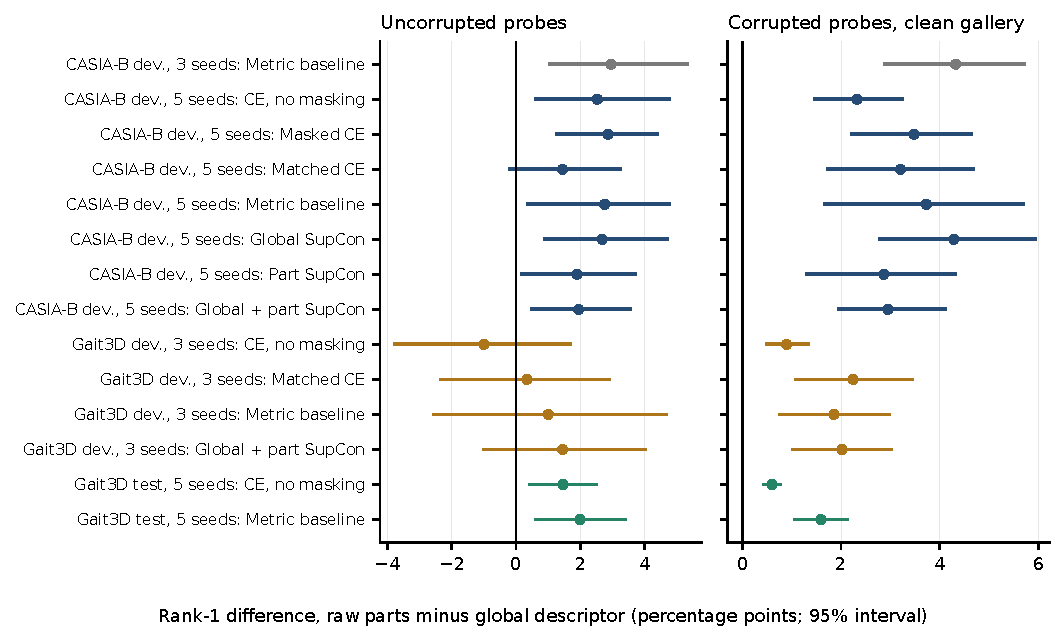
\includegraphics[width=0.82\textwidth]{fig3.pdf}
\caption{Raw reliability-weighted part matching minus global matching (Rank-1
points, crossed 95\% bootstrap intervals) for every cohort and training
objective. The corrupted-probe panel averages four families at severities
0.1--0.7. Exact values are listed in Supplementary Table~S6.}
\label{fig:forest}
\end{figure*}

\begin{figure*}[!t]
\centering
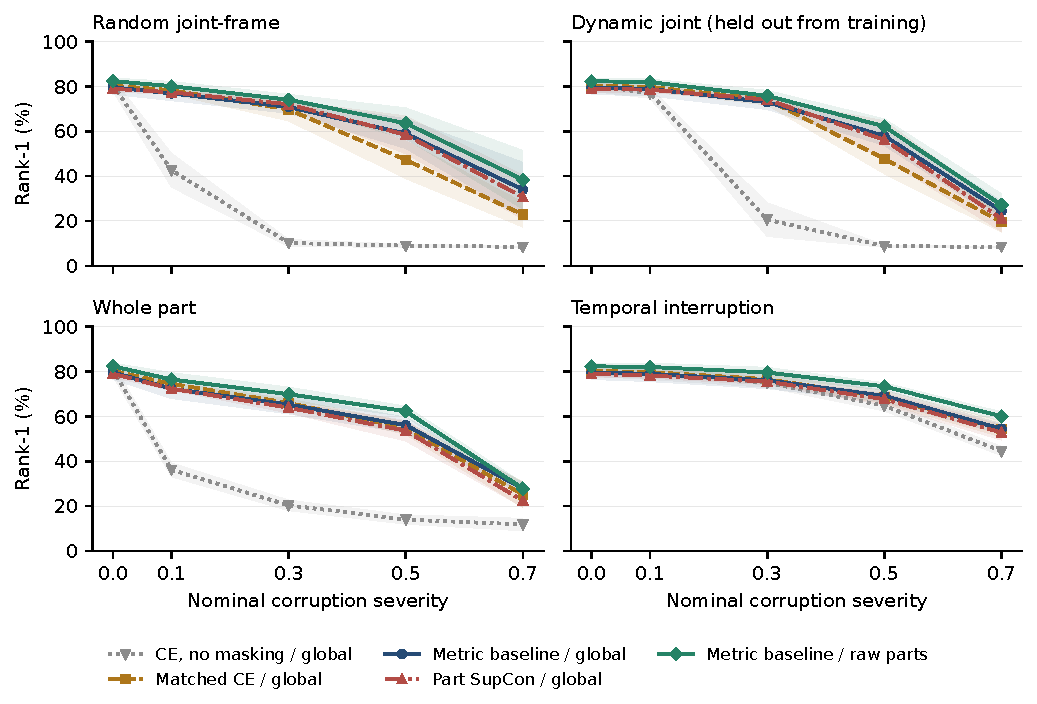
\includegraphics[width=0.82\textwidth]{fig4.pdf}
\caption{CASIA-B development severity curves with a clean gallery. Lines are
means over five training seeds and shaded bands one seed standard deviation.
Positive severities average five mask realizations. Severity is nominal and
does not imply equal removed fractions across families.}
\label{fig:severity}
\end{figure*}

\subsection{CASIA-B official test}

Only the metric baseline was retrained on all 74 training identities, for a
fixed 85 epochs (the median selected development epoch, fixed before these
runs), with five seeds. On the standard protocol (Table~\ref{tab:main}),
raw reliability-weighted parts raise the NM/BG/CL average from
$48.35\pm1.85$\% to $54.04\pm2.18$\%, a paired gain of 5.69 points with interval
$[5.19,6.20]$; the gains are 6.50 points for NM, 5.97 for BG and 4.61 for CL,
and every seed improves (5.05 to 6.02 points); uniform and reliability-weighted
fusion differ by $+0.004$ points (Supplementary Table~S10 gives the
per-condition spread). The absolute level is low: GPGait reproduced on the same
split reaches 80.91\%, within 0.1 points of its reported 81.01\%, and even our
GaitGraph2 reproduction (68.17\%, 3.66 points below its reported value) exceeds
our encoder.

\begin{table*}[!t]
\centering
\caption{Test-set comparison, Rank-1 and mAP (\%). CASIA-B uses identities
075--124 with the standard single-view protocol excluding identical views;
Gait3D uses the available-pose subset (947 probes, 5,122 gallery sequences),
evaluated once with the recipe frozen on development data. Our rows are means
over five seeds of the metric baseline; reproduced baselines were trained once
with official FastPoseGait configurations, and reported values are those of the
FastPoseGait model zoo \cite{meng2023fastposegait} on the complete benchmarks.
Panel (b) rescores the same GPGait checkpoints (full: all 19 embeddings); raw
parts are fused at $\lambda=0.5$. Parameter counts include identity
classifiers. Standard deviations, further metrics and paired intervals are in
Supplementary Tables~S10--S12.}
\label{tab:main}
{\tablesetup\setlength{\tabcolsep}{2.5pt}
\begin{tabular}{@{}lccccccc@{}}
\toprule
 & \multicolumn{4}{c}{CASIA-B official test} & \multicolumn{2}{c}{Gait3D test} & \\
\cmidrule(lr){2-5}\cmidrule(lr){6-7}
System & NM & BG & CL & Avg. & Rank-1 & mAP & \begin{tabular}[b]{@{}c@{}}Params. (M)\\CASIA / G3D\end{tabular} \\
\midrule
\multicolumn{8}{@{}l}{\emph{(a) Systems}} \\
Ours, global (5 runs) & $67.64$ & $49.50$ & $27.91$ & $48.35$ & $21.88$ & $16.89$ & 1.69 / 2.41 \\
Ours, raw parts (5 runs) & $74.14$ & $55.47$ & $32.52$ & $54.04$ & $23.86$ & $17.79$ & 1.69 / 2.41 \\
GaitGraph2, reproduced & $76.66$ & $67.23$ & $60.63$ & $68.17$ & $8.87$ & $8.38$ & 0.35 / 0.35 \\
GaitGraph2, reported & $80.29$ & $71.40$ & $63.80$ & $71.83$ & $11.20$ & -- & -- \\
GPGait, reproduced & $93.77$ & $79.86$ & $69.11$ & $80.91$ & $23.13$ & $16.78$ & 3.65 / 18.11 \\
GPGait, reported & $93.60$ & $80.15$ & $69.29$ & $81.01$ & $22.40$ & -- & -- \\
\midrule
\multicolumn{8}{@{}l}{\emph{(b) GPGait descriptor variants (same checkpoints)}} \\
Whole-body only & $87.86$ & $68.21$ & $59.49$ & $71.85$ & $17.95$ & $12.59$ &  \\
Whole-body + raw parts & $86.53$ & $67.15$ & $59.07$ & $70.92$ & $17.11$ & $11.86$ &  \\
Full + raw parts & $91.55$ & $77.01$ & $67.05$ & $78.53$ & $19.96$ & $14.24$ &  \\
\bottomrule
\end{tabular}}
\end{table*}

\subsection{External evaluation on Gait3D}

Table~\ref{tab:main} reports the single test evaluation. With the frozen
recipe, raw reliability-weighted parts raise the metric baseline's Rank-1 from
$21.88\pm1.18$\% to $23.86\pm0.68$\%, a paired gain of 1.99 points with crossed
interval $[0.61,3.38]$, and mAP from 16.89\% to 17.79\%. The gain is also present
on corrupted probes (1.59 points, $[1.07,2.12]$), with corrupted galleries
(1.19, $[0.76,1.63]$) and for the CE model (1.46 clean points,
$[0.44,2.47]$). For the metric baseline, reliability and uniform weighting
coincide to within 0.02 points on every endpoint. The metric baseline exceeds CE by 6.40 clean points,
$[4.18,8.76]$, and 10.62 corrupted-probe points, confirming the development
ranking on unseen identities. GPGait trained on the identical subset reaches
23.13\% Rank-1 and 16.78\% mAP with 18.11 M parameters, against 23.86\% and
17.79\% for the 2.41 M-parameter encoder with raw parts; our GaitGraph2
reproduction reaches 8.87\%. Because each baseline was trained once and scored
by its own evaluator, we read this as parity with GPGait on this subset rather
than as an advantage (Rank-5, Rank-10 and mINP are in Supplementary
Table~S11).

\paragraph{Real detector confidence}
Gait3D has no occlusion labels, so we stratified development probes by the
fraction of joint-frames with HRNet confidence below 0.5, a proxy fixed before
outcomes were examined (Supplementary Section~S7). The pre-specified
height-matched contrast of the raw-minus-global gain between the most and least
low-confidence tertiles is $-0.68$ points, $[-7.69,6.22]$: the gain is not
concentrated on low-confidence probes, and these data cannot show that it
addresses real occlusion.

\subsection{Transfer to GPGait}

Table~\ref{tab:main}(b) applies the matcher to GPGait (paired intervals in
Supplementary Table~S12). Unlike in our encoder, GPGait's trained part branches
carry much of its accuracy: removing them lowers the CASIA-B average by 9.08
points, $[7.43,10.71]$, and Gait3D Rank-1 by 5.17, $[3.06,7.29]$. Raw parts
neither replace nor complement them: fused with the whole-body descriptor they
change the average by $-0.94$, $[-1.77,-0.15]$, and fused with the full
descriptor they lower it by 2.40, $[1.53,3.29]$, and Gait3D Rank-1 by 3.17,
$[1.80,4.65]$. An exploratory variant chosen after these results, which projects
mean-plus-max region pools through each branch's trained whole-body head, also
improves neither fusion (Supplementary Table~S9). This agrees with GPGait's own
ablation, in which removing the partition masks at equal parameter count
lowered CASIA-B accuracy from 81.01\% to 76.47\% and Gait3D Rank-1 from 22.40\%
to 20.40\% \cite{fu2023gpgait}.

\subsection{Cost}

The encoder uses 1.54 M parameters at inference and encodes a 48-frame sequence
in $4.06\pm0.07$ ms at batch size one on a one-seventh H100 NVL partition (MIG
1g.12gb), excluding gallery matching. Raw parts add no parameters but store
1,536 coordinates and five reliabilities per sequence instead of 256. The
reproduced baselines were not timed, so no speed comparisons are made.

\section{Discussion}
\label{sec:discussion}

\paragraph{Which part intervention helps depends on the encoder}
In our encoder, auxiliary part supervision did not help and untrained regional
pools did; in GPGait, part-specific branches trained with their own losses
added 5 to 9 points and raw pools added nothing. The results need not conflict:
our part SupCon was an auxiliary loss on shared features, whereas GPGait trains
separate branches with restricted connectivity, and raw pools can only add
evidence the global embedding lacks. Without both comparisons either intervention
could be credited wrongly, so global, raw regional and trained regional matching
should be compared on the same frozen checkpoint. Replication also mattered: a
part-SupCon penalty supported by three seeds and 12 identities did not survive
five seeds.

\paragraph{What the matching gain is and is not}
Uniform and reliability-weighted fusion are indistinguishable, and random
heads help less than raw pools, so neither confidence gating nor a learned
projection is required. Without size-matched random regions the gain is tied to
regional score fusion, not to anatomical grouping as such. It is smaller on
Gait3D than on CASIA-B and not concentrated on low-confidence probes, so it may
reflect a generic ensembling benefit as much as robustness to missing parts.

\paragraph{Absolute performance and silhouettes}
With raw parts our encoder matches GPGait on Gait3D but is 27 points below it
on CASIA-B, and raw matching does not improve GPGait itself, so the matcher is a
cheap remedy for encoders whose regional features were not trained for
retrieval rather than a way to improve strong part-aware systems.
Silhouette-based systems remain more accurate still
\cite{chao2019gaitset,fan2020gaitpart,lin2021gaitgl,fan2022opengait}, because
silhouettes keep body shape that keypoints discard \cite{fu2023gpgait}; pose is
compact, less affected by clothing and carried objects, and makes body regions
explicit. Silhouette models usually train horizontal part strips with their own
losses \cite{chao2019gaitset,fan2020gaitpart}; whether raw regional matching
behaves there as in our encoder or as in GPGait is untested.

\paragraph{Outlook}
Cross-dataset evaluation, the focus of GPGait \cite{fu2023gpgait}, would test
whether raw regional matching helps across cameras and environments; labelled
real occlusion such as the SUSTech1K occlusion condition \cite{shen2023lidargait}
and larger pose datasets such as OU-MVLP-Pose and GREW
\cite{an2020oumvlppose,zhu2021grew} would test the occlusion and scale claims;
and because the matcher needs no training, it could aid pseudo-labelling of
unlabelled gait data by clustering self-supervised contrastive embeddings
\cite{cosma2026gaitpt}.

\section{Limitations}
\label{sec:limitations}

\paragraph{Data and exposure}
CASIA-B development comparisons rest on 12 identities, and its test identities
were examined in earlier project experiments. Gait3D test identities are
unexposed, but cover only the metric baseline and CE on an available-pose
subset lacking 53 test identities.

\paragraph{Synthetic and proxy occlusion}
Masks applied after normalization omit left--right swaps, cross-person
assignments, wrong tracks and occlusion-induced normalization errors, detector
confidence is only a proxy for occlusion, and labelled real occlusion was not
used.

\paragraph{One encoder and fixed settings}
All objectives share one encoder, pose source, loss weights and temperatures,
so tuning or other part objectives could change the ranking; random-region
controls are absent.

\paragraph{Baselines and statistics}
External baselines were trained once and scored by their own evaluators; our
GaitGraph2 reproduction fell 2.3 to 3.7 points short. The GPGait test uses clean
probes, and removing its part branches removes their architecture and losses
together. Many comparisons are exploratory and intervals unadjusted.

\paragraph{Ethical considerations}
Gait can identify people without their awareness; robustness gains do not
remove the need for a lawful purpose, consent where applicable, access control,
retention limits and human oversight, and these datasets support neither
fairness nor deployment claims. Operational evaluation should follow
established biometric testing principles such as ISO/IEC 19795-1
\cite{iso19795}.

\section{Conclusion}
\label{sec:conclusion}

On our encoder, auxiliary SupCon objectives did not reliably change accuracy,
whereas raw part matching from frozen checkpoints improved corrupted-probe
Rank-1 under every objective and raised Gait3D test Rank-1 by 1.99 points,
$[0.61,3.38]$, to parity with GPGait; on GPGait, trained part branches added 5 to
9 points and raw matching lowered accuracy. Where a part-aware gain comes from
is therefore encoder-dependent, and part-aware systems should report global,
raw regional and trained regional matching on the same frozen checkpoints.


\section*{Ethics Statement}
This study analyses only publicly released benchmark data, CASIA-B and Gait3D,
which were collected and distributed by their creators under their own
protocols and licences. No new data involving human participants were collected
and no participant was contacted.

\section*{Data and Code Availability}
CASIA-B poses are the HRNet-derived release distributed through FastPoseGait
(\url{https://github.com/BNU-IVC/FastPoseGait}); the dataset is available from
Science Data Bank
(\url{https://www.scidb.cn/en/detail?dataSetId=8ec62efd66a544939e821edeccc1f35c}).
Gait3D and its 2D poses are available from the dataset authors
(\url{https://gait3d.github.io/}) under their licence. Neither dataset is
redistributed. Identity splits, preprocessing, corruption seeds, per-probe
outcomes and the scripts that regenerate every table and figure are available
with the code at \url{https://github.com/likwifi/oap-supcon}.

\section*{Acknowledgment}
The authors used Claude (Anthropic) to assist with analysis scripting,
consolidation of experimental results and editing of the manuscript text. The
authors reviewed and edited all such content and take full responsibility for
the article.

% Bibliography generated with IEEEtran.bst from references.bib.
% Generated by IEEEtran.bst, version: 1.14 (2015/08/26)
\begin{thebibliography}{10}
\providecommand{\url}[1]{#1}
\csname url@samestyle\endcsname
\providecommand{\newblock}{\relax}
\providecommand{\bibinfo}[2]{#2}
\providecommand{\BIBentrySTDinterwordspacing}{\spaceskip=0pt\relax}
\providecommand{\BIBentryALTinterwordstretchfactor}{4}
\providecommand{\BIBentryALTinterwordspacing}{\spaceskip=\fontdimen2\font plus
\BIBentryALTinterwordstretchfactor\fontdimen3\font minus
  \fontdimen4\font\relax}
\providecommand{\BIBforeignlanguage}[2]{{%
\expandafter\ifx\csname l@#1\endcsname\relax
\typeout{** WARNING: IEEEtran.bst: No hyphenation pattern has been}%
\typeout{** loaded for the language `#1'. Using the pattern for}%
\typeout{** the default language instead.}%
\else
\language=\csname l@#1\endcsname
\fi
#2}}
\providecommand{\BIBdecl}{\relax}
\BIBdecl

\bibitem{liao2020posegait}
R.~Liao, S.~Yu, W.~An, and Y.~Huang, ``A model-based gait recognition method
  with body pose and human prior knowledge,'' \emph{{Pattern Recognition}},
  vol.~98, p. 107069, 2020.

\bibitem{yan2018stgcn}
S.~Yan, Y.~Xiong, and D.~Lin, ``Spatial temporal graph convolutional networks
  for skeleton-based action recognition,'' in \emph{{Proceedings of the AAAI
  Conference on Artificial Intelligence}}, vol.~32, 2018.

\bibitem{teepe2021gaitgraph}
T.~Teepe, A.~Khan, J.~Gilg, F.~Herzog, S.~H{\"o}rmann, and G.~Rigoll,
  ``{GaitGraph}: Graph convolutional network for skeleton-based gait
  recognition,'' in \emph{{2021 IEEE International Conference on Image
  Processing}}, 2021, pp. 2314--2318.

\bibitem{teepe2022gaitgraph2}
T.~Teepe, J.~Gilg, F.~Herzog, S.~H{\"o}rmann, and G.~Rigoll, ``Towards a deeper
  understanding of skeleton-based gait recognition,'' in \emph{{Proceedings of
  the IEEE/CVF Conference on Computer Vision and Pattern Recognition
  Workshops}}, 2022, pp. 1569--1577.

\bibitem{li2024survey}
T.~Li, W.~Ma, Y.~Zheng, X.~Fan, G.~Yang, L.~Wang, and Z.~Li, ``A survey on gait
  recognition against occlusion: Taxonomy, dataset and methodology,''
  \emph{{PeerJ Computer Science}}, vol.~10, p. e2602, 2024.

\bibitem{huang2024occluded}
P.~Huang, Y.~Peng, S.~Hou, C.~Cao, X.~Liu, Z.~He, and Y.~Huang, ``Occluded gait
  recognition with mixture of experts: An action detection perspective,'' in
  \emph{{Proceedings of the European Conference on Computer Vision}}, 2024, pp.
  380--397.

\bibitem{khosla2020supervised}
P.~Khosla, P.~Teterwak, C.~Wang, A.~Sarna, Y.~Tian, P.~Isola, A.~Maschinot,
  C.~Liu, and D.~Krishnan, ``Supervised contrastive learning,'' in
  \emph{{Advances in Neural Information Processing Systems}}, vol.~33, 2020,
  pp. 18\,661--18\,673.

\bibitem{fu2023gpgait}
Y.~Fu, S.~Meng, S.~Hou, X.~Hu, and Y.~Huang, ``{GPGait}: Generalized pose-based
  gait recognition,'' in \emph{{Proceedings of the IEEE/CVF International
  Conference on Computer Vision}}, 2023, pp. 19\,595--19\,604.

\bibitem{chen2020simclr}
T.~Chen, S.~Kornblith, M.~Norouzi, and G.~Hinton, ``A simple framework for
  contrastive learning of visual representations,'' in \emph{{Proceedings of
  the 37th International Conference on Machine Learning}}, ser. Proceedings of
  Machine Learning Research, vol. 119, 2020, pp. 1597--1607.

\bibitem{he2020moco}
K.~He, H.~Fan, Y.~Wu, S.~Xie, and R.~Girshick, ``Momentum contrast for
  unsupervised visual representation learning,'' in \emph{{Proceedings of the
  IEEE/CVF Conference on Computer Vision and Pattern Recognition}}, 2020, pp.
  9729--9738.

\bibitem{wang2020alignment}
T.~Wang and P.~Isola, ``{Understanding Contrastive Representation Learning
  through Alignment and Uniformity on the Hypersphere},'' in \emph{{Proceedings
  of the 37th International Conference on Machine Learning}}, ser. Proceedings
  of Machine Learning Research, vol. 119, 2020, pp. 9929--9939.

\bibitem{grill2020byol}
J.-B. Grill, F.~Strub, F.~Altch{\'e}, C.~Tallec, P.~Richemond, E.~Buchatskaya,
  C.~Doersch, B.~A. Pires, Z.~Guo, M.~G. Azar, B.~Piot, K.~Kavukcuoglu,
  R.~Munos, and M.~Valko, ``{Bootstrap Your Own Latent - A New Approach to
  Self-Supervised Learning},'' in \emph{{Advances in Neural Information
  Processing Systems}}, vol.~33, 2020.

\bibitem{chen2021simsiam}
X.~Chen and K.~He, ``{Exploring Simple Siamese Representation Learning},'' in
  \emph{{Proceedings of the IEEE/CVF Conference on Computer Vision and Pattern
  Recognition}}, 2021, pp. 15\,750--15\,758.

\bibitem{zbontar2021barlow}
J.~Zbontar, L.~Jing, I.~Misra, Y.~LeCun, and S.~Deny, ``{Barlow Twins:
  Self-Supervised Learning via Redundancy Reduction},'' in \emph{{Proceedings
  of the 38th International Conference on Machine Learning}}, ser. Proceedings
  of Machine Learning Research, vol. 139, 2021, pp. 12\,310--12\,320.

\bibitem{bardes2022vicreg}
A.~Bardes, J.~Ponce, and Y.~LeCun, ``{VICReg: Variance-Invariance-Covariance
  Regularization for Self-Supervised Learning},'' in \emph{{International
  Conference on Learning Representations}}, 2022.

\bibitem{thoker2021skeleton}
F.~M. Thoker, H.~Doughty, and C.~G.~M. Snoek, ``Skeleton-contrastive 3d action
  representation learning,'' in \emph{{Proceedings of the 29th ACM
  International Conference on Multimedia}}, 2021, pp. 1655--1663.

\bibitem{rao2024skeleton}
H.~Rao and C.~Miao, ``Skeleton prototype contrastive learning with multi-level
  graph relation modeling for unsupervised person re-identification,'' in
  \emph{{Quality, Reliability, Security and Robustness in Heterogeneous
  Systems}}.\hskip 1em plus 0.5em minus 0.4em\relax Springer, 2024, pp.
  306--321.

\bibitem{lin2023actclr}
L.~Lin, J.~Zhang, and J.~Liu, ``{Actionlet-Dependent Contrastive Learning for
  Unsupervised Skeleton-Based Action Recognition},'' in \emph{{Proceedings of
  the IEEE/CVF Conference on Computer Vision and Pattern Recognition}}, 2023,
  pp. 2363--2372.

\bibitem{cosma2026gaitpt}
A.~Cosma, A.~E. Catruna, and E.~Radoi, ``On model and data scaling for
  skeleton-based self-supervised gait recognition,'' in \emph{{Proceedings of
  the AAAI Conference on Artificial Intelligence}}, vol.~40, 2026, pp.
  3434--3442.

\bibitem{wu2017sampling}
C.-Y. Wu, R.~Manmatha, A.~J. Smola, and P.~Krahenbuhl, ``{Sampling Matters in
  Deep Embedding Learning},'' in \emph{{Proceedings of the IEEE/CVF
  International Conference on Computer Vision}}, 2017, pp. 2840--2848.

\bibitem{wang2019multisimilarity}
X.~Wang, X.~Han, W.~Huang, D.~Dong, and M.~R. Scott, ``{Multi-Similarity Loss
  With General Pair Weighting for Deep Metric Learning},'' in
  \emph{{Proceedings of the IEEE/CVF Conference on Computer Vision and Pattern
  Recognition}}, 2019, pp. 5022--5030.

\bibitem{musgrave2020reality}
K.~Musgrave, S.~Belongie, and S.-N. Lim, ``{A Metric Learning Reality Check},''
  in \emph{{Computer Vision -- ECCV 2020}}, 2020, pp. 681--699.

\bibitem{sener2018multiobjective}
O.~Sener and V.~Koltun, ``{Multi-Task Learning as Multi-Objective
  Optimization},'' in \emph{{Advances in Neural Information Processing
  Systems}}, vol.~31, 2018.

\bibitem{yu2020gradient}
T.~Yu, S.~Kumar, A.~Gupta, S.~Levine, K.~Hausman, and C.~Finn, ``{Gradient
  Surgery for Multi-Task Learning},'' in \emph{{Advances in Neural Information
  Processing Systems}}, vol.~33, 2020.

\bibitem{fan2024skeletongait}
C.~Fan, J.~Ma, D.~Jin, C.~Shen, and S.~Yu, ``{SkeletonGait}: Gait recognition
  using skeleton maps,'' in \emph{{Proceedings of the AAAI Conference on
  Artificial Intelligence}}, vol.~38, 2024, pp. 1662--1669.

\bibitem{fan2022opengait}
C.~Fan, J.~Liang, C.~Shen, S.~Hou, Y.~Huang, and S.~Yu, ``{OpenGait}:
  Revisiting gait recognition toward better practicality,'' in
  \emph{{Proceedings of the IEEE/CVF Conference on Computer Vision and Pattern
  Recognition}}, 2023, pp. 9707--9716.

\bibitem{meng2023fastposegait}
S.~Meng, Y.~Fu, S.~Hou, C.~Cao, X.~Liu, and Y.~Huang, ``{FastPoseGait}: A
  toolbox and benchmark for efficient pose-based gait recognition,''
  \emph{arXiv preprint arXiv:2309.00794}, 2023.

\bibitem{shi2019adaptive}
L.~Shi, Y.~Zhang, J.~Cheng, and H.~Lu, ``{Two-Stream Adaptive Graph
  Convolutional Networks for Skeleton-Based Action Recognition},'' in
  \emph{{Proceedings of the IEEE/CVF Conference on Computer Vision and Pattern
  Recognition}}, 2019, pp. 12\,026--12\,035.

\bibitem{li2019actional}
M.~Li, S.~Chen, X.~Chen, Y.~Zhang, Y.~Wang, and Q.~Tian, ``{Actional-Structural
  Graph Convolutional Networks for Skeleton-Based Action Recognition},'' in
  \emph{{Proceedings of the IEEE/CVF Conference on Computer Vision and Pattern
  Recognition}}, 2019, pp. 3595--3603.

\bibitem{liu2020msg3d}
Z.~Liu, H.~Zhang, Z.~Chen, Z.~Wang, and W.~Ouyang, ``{Disentangling and
  Unifying Graph Convolutions for Skeleton-Based Action Recognition},'' in
  \emph{{Proceedings of the IEEE/CVF Conference on Computer Vision and Pattern
  Recognition}}, 2020, pp. 143--152.

\bibitem{cheng2020shift}
K.~Cheng, Y.~Zhang, X.~He, W.~Chen, J.~Cheng, and H.~Lu, ``{Skeleton-Based
  Action Recognition With Shift Graph Convolutional Network},'' in
  \emph{{Proceedings of the IEEE/CVF Conference on Computer Vision and Pattern
  Recognition}}, 2020, pp. 183--192.

\bibitem{duan2022posec3d}
H.~Duan, Y.~Zhao, K.~Chen, D.~Lin, and B.~Dai, ``{Revisiting Skeleton-Based
  Action Recognition},'' in \emph{{Proceedings of the IEEE/CVF Conference on
  Computer Vision and Pattern Recognition}}, 2022, pp. 2969--2978.

\bibitem{chen2023iopstl}
Y.~Chen, K.~Peng, A.~Roitberg, D.~Schneider, J.~Zhang, J.~Zheng, Y.~Chen,
  R.~Liu, K.~Yang, and R.~Stiefelhagen, ``Exploring self-supervised
  skeleton-based action recognition in occluded environments,'' \emph{{arXiv
  preprint arXiv:2309.12029}}, 2023.

\bibitem{zhu2021grew}
Z.~Zhu, X.~Guo, T.~Yang, J.~Huang, J.~Deng, G.~Huang, D.~Du, J.~Lu, and
  J.~Zhou, ``Gait recognition in the wild: A benchmark,'' in \emph{{Proceedings
  of the IEEE/CVF International Conference on Computer Vision}}, 2021, pp.
  14\,789--14\,799.

\bibitem{zheng2022gait3d}
J.~Zheng, X.~Liu, W.~Liu, L.~He, C.~Yan, and T.~Mei, ``Gait recognition in the
  wild with dense 3d representations and a benchmark,'' in \emph{{Proceedings
  of the IEEE/CVF Conference on Computer Vision and Pattern Recognition}},
  2022, pp. 20\,228--20\,237.

\bibitem{shen2023lidargait}
C.~Shen, C.~Fan, W.~Wu, R.~Wang, G.~Q. Huang, and S.~Yu, ``{LidarGait:
  Benchmarking 3D Gait Recognition With Point Clouds},'' in \emph{{Proceedings
  of the IEEE/CVF Conference on Computer Vision and Pattern Recognition}},
  2023, pp. 1054--1063.

\bibitem{chao2019gaitset}
H.~Chao, Y.~He, J.~Zhang, and J.~Feng, ``{GaitSet: Regarding Gait as a Set for
  Cross-View Gait Recognition},'' in \emph{{Proceedings of the AAAI Conference
  on Artificial Intelligence}}, vol.~33, 2019, pp. 8126--8133.

\bibitem{zhang2019disentangled}
Z.~Zhang, L.~Tran, X.~Yin, Y.~Atoum, X.~Liu, J.~Wan, and N.~Wang, ``{Gait
  Recognition via Disentangled Representation Learning},'' in
  \emph{{Proceedings of the IEEE/CVF Conference on Computer Vision and Pattern
  Recognition}}, 2019, pp. 4710--4719.

\bibitem{li2020disentangled}
X.~Li, Y.~Makihara, C.~Xu, Y.~Yagi, and M.~Ren, ``{Gait Recognition via
  Semi-supervised Disentangled Representation Learning to Identity and
  Covariate Features},'' in \emph{{Proceedings of the IEEE/CVF Conference on
  Computer Vision and Pattern Recognition}}, 2020, pp. 13\,309--13\,319.

\bibitem{fan2020gaitpart}
C.~Fan, Y.~Peng, C.~Cao, X.~Liu, S.~Hou, J.~Chi, Y.~Huang, Q.~Li, and Z.~He,
  ``{GaitPart}: Temporal part-based model for gait recognition,'' in
  \emph{{Proceedings of the IEEE/CVF Conference on Computer Vision and Pattern
  Recognition}}, 2020, pp. 14\,225--14\,233.

\bibitem{lin2021gaitgl}
B.~Lin, S.~Zhang, and X.~Yu, ``Gait recognition via effective global-local
  feature representation and local temporal aggregation,'' in
  \emph{{Proceedings of the IEEE/CVF International Conference on Computer
  Vision}}, 2021, pp. 14\,648--14\,656.

\bibitem{huang2021local}
Z.~Huang, D.~Xue, X.~Shen, X.~Tian, H.~Li, J.~Huang, and X.-S. Hua, ``3d local
  convolutional neural networks for gait recognition,'' in \emph{{Proceedings
  of the IEEE/CVF International Conference on Computer Vision}}, 2021, pp.
  14\,920--14\,929.

\bibitem{wang2022gaitstrip}
M.~Wang, B.~Lin, X.~Guo, L.~Li, Z.~Zhu, J.~Sun, S.~Zhang, Y.~Liu, and X.~Yu,
  ``{GaitStrip: Gait Recognition via Effective Strip-based Feature
  Representations and Multi-Level Framework},'' in \emph{{Proceedings of the
  Asian Conference on Computer Vision}}, 2022, pp. 536--551.

\bibitem{huang2021cstl}
X.~Huang, D.~Zhu, H.~Wang, X.~Wang, B.~Yang, B.~He, W.~Liu, and B.~Feng,
  ``{Context-Sensitive Temporal Feature Learning for Gait Recognition},'' in
  \emph{{Proceedings of the IEEE/CVF International Conference on Computer
  Vision}}, 2021, pp. 12\,909--12\,918.

\bibitem{wang2023dygait}
M.~Wang, X.~Guo, B.~Lin, T.~Yang, Z.~Zhu, L.~Li, S.~Zhang, and X.~Yu,
  ``{DyGait: Exploiting Dynamic Representations for High-performance Gait
  Recognition},'' in \emph{{Proceedings of the IEEE/CVF International
  Conference on Computer Vision}}, 2023, pp. 13\,424--13\,433.

\bibitem{huang2025template}
P.~Huang, S.~Hou, J.~Huang, and Y.~Huang, ``{Learning A Unified Template for
  Gait Recognition},'' in \emph{{Proceedings of the IEEE/CVF International
  Conference on Computer Vision}}, 2025, pp. 12\,459--12\,469.

\bibitem{hermans2017triplet}
A.~Hermans, L.~Beyer, and B.~Leibe, ``In defense of the triplet loss for person
  re-identification,'' \emph{{arXiv preprint arXiv:1703.07737}}, 2017.

\bibitem{sun2019hrnet}
K.~Sun, B.~Xiao, D.~Liu, and J.~Wang, ``Deep high-resolution representation
  learning for human pose estimation,'' in \emph{{Proceedings of the IEEE/CVF
  Conference on Computer Vision and Pattern Recognition}}, 2019, pp.
  5693--5703.

\bibitem{yu2006casia}
S.~Yu, D.~Tan, and T.~Tan, ``A framework for evaluating the effect of view
  angle, clothing and carrying condition on gait recognition,'' in \emph{{18th
  International Conference on Pattern Recognition}}, 2006, pp. 441--444.

\bibitem{lin2014coco}
T.-Y. Lin, M.~Maire, S.~Belongie, J.~Hays, P.~Perona, D.~Ramanan,
  P.~Doll{\'a}r, and C.~L. Zitnick, ``Microsoft {COCO}: Common objects in
  context,'' in \emph{{Computer Vision -- ECCV 2014}}, 2014, pp. 740--755.

\bibitem{an2020oumvlppose}
W.~An, S.~Yu, Y.~Makihara, X.~Wu, C.~Xu, Y.~Yu, R.~Liao, and Y.~Yagi,
  ``Performance evaluation of model-based gait on multi-view very large
  population database with pose sequences,'' \emph{IEEE Transactions on
  Biometrics, Behavior, and Identity Science}, vol.~2, no.~4, pp. 421--430,
  2020.

\bibitem{iso19795}
{ISO/IEC}, ``Information technology -- biometric performance testing and
  reporting -- part 1: Principles and framework,'' International Standard
  ISO/IEC 19795-1:2021, 2021.

\end{thebibliography}

\end{document}
